\documentclass[crop,tikz]{standalone}
\usetikzlibrary{backgrounds}
\colorlet{blue}{cyan}
\tikzset{
  inverted/.style = {
    color=white,
    background rectangle/.style={fill},
    show background rectangle
  }
}

\usepackage{pgfplots}
\tikzset{>=latex}

\pgfplotsset{
  inverted/.style = {
    every axis legend/.append style={
      draw=white,
      fill=black,
      text=white
    }
  }
}

\begin{document}
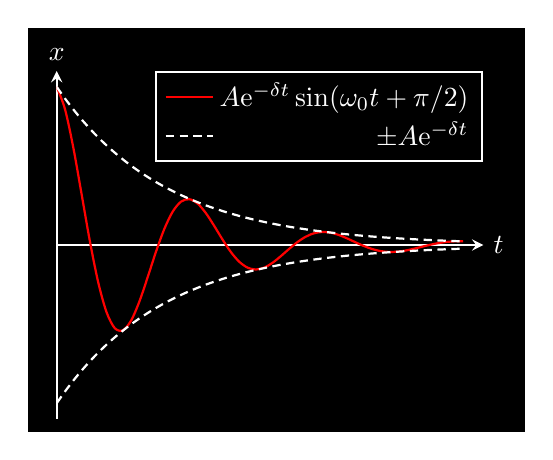
\begin{tikzpicture}[inverted,inverted]
\pgfmathsetmacro{\damp}{0.2}
\begin{axis}[inverted,
  thick,
  width=7cm,
  height=6cm,
  domain={0}:{6*pi},
  samples=50,
  axis y line=middle,
  axis x line=middle,
  xlabel={$t$},
  ylabel={$x$},
  xlabel style={right},
  ylabel style={above},
  xmin=0, xmax={6.3*pi},
  ymin=-1.1, ymax=1.1,
  xtick={\empty},
  xticklabels={\empty},
  ytick={\empty},
  yticklabels={\empty},
  legend cell align={right},
  legend style={at={(1,1)},anchor=north east}
  ]
  \addplot[red,smooth] { exp(-\damp*x)*cos(deg(x)) };
  \addlegendentry{$A \mathrm{e}^{-\delta t} \sin(\omega_0 t + \pi/2)$};
  \addplot[smooth,densely dashed] { exp(-\damp*x) };
  \addplot[smooth,densely dashed] { -exp(-\damp*x) };
  \addlegendentry{$\pm A \mathrm{e}^{-\delta t}$};
\end{axis}
\end{tikzpicture}
\end{document}
